%%%%%%%%%%%%%%%%%%%%%%%%%%%%%%%%%%%%%%%%%%%%%%%%%%%%%%%%%%%%%%%%%%%%%%%%%%%%%%%%
% How_to_Transform_the_World_MVL_EN.tex
% Compile with: xelatex or pdflatex (twice for references)
% Requires: amsmath, amssymb, booktabs, graphicx, hyperref, pgfplots, tikz
%%%%%%%%%%%%%%%%%%%%%%%%%%%%%%%%%%%%%%%%%%%%%%%%%%%%%%%%%%%%%%%%%%%%%%%%%%%%%%%%

\documentclass[11pt,a4paper]{article}

\usepackage[utf8]{inputenc}
\usepackage[T1]{fontenc}
\usepackage{geometry}
\geometry{margin=2.5cm}
\usepackage{amsmath,amssymb,amsfonts}
\usepackage{booktabs}
\usepackage{graphicx}
\usepackage{xcolor}
\usepackage{hyperref}
\usepackage{pgfplots}
\pgfplotsset{compat=1.18}
\usepackage{tikz}
\usetikzlibrary{shapes.geometric, arrows.meta, positioning, calc}

\title{\bfseries Transforming the World through the Median Value Law:\\
A Quantum--Classical Framework for Hierarchical Recomposition}

\author{
Xiaohui Li\\
Independent Researcher, Baoji 721000, China\\
\textit{Correspondence:} danceluck@163.com\\
ORCID: 0009-0003-8233-7191\\
Data and code: \url{https://github.com/xiaohui-li-lab/}
}
\date{}

\begin{document}

\maketitle

\begin{abstract}
\noindent
We present a transdisciplinary framework---the Median Value Law (MVL)---that integrates three questions about intelligence and world-transformation: the ``hardware'' of information processing, the ``software'' of decomposition--recomposition, and the optimal scale at which to intervene in a hierarchical system. Drawing on neuroscience, quantum biology, complex systems, and contemplative epistemology, we argue that intelligent systems operate through three cumulative layers: socio-empirical, sensory-decompositional, and quantum-recombinatorial. The central thesis of the MVL posits that the most efficient locus of systemic change lies not at the smallest or largest scale, but at an intermediate ``median'' scale---often approximated by the golden ratio---from which perturbations propagate bidirectionally to microscopic and macroscopic levels. Using publicly available cosmological and anthropometric data, we derive a testable scaling relation that anchors the human scale between the Planck length and the observable Universe. We validate the principle with a multi-scale network simulation showing that, when causal weighting is centred on the organism scale, interventions at or near the human scale maximize global influence. The framework generates falsifiable predictions in quantum cognition, complex systems, and cosmology, and provides open datasets and code for replication.
\end{abstract}

\noindent\textbf{Keywords:} Median value law; quantum cognition; hierarchical decomposition; golden ratio; scale invariance; complex systems; human-scale universe; integrated information; cardiac-blood quantum channel; infrared information processing.

\section{Introduction}

Understanding intelligence and its capacity to transform the world requires more than a theory of neurons. It demands a theory of how information is processed, how phenomena are decomposed and recomposed, and where in the hierarchy of scales an intervention can most efficiently propagate [1,2]. Contemporary artificial intelligence has excelled at neural computation, yet it remains largely silent on the questions of scale, embodiment, and the recursive restructuring of reality that characterize human wisdom [3,4].

Here we introduce the Median Value Law (MVL), a transdisciplinary framework that formalizes three interlocking problems. First, cognitive ``hardware'': the channels through which information flows. Second, cognitive ``software'': the operations by which experience is analysed and synthesized. Third, a scale-invariant intervention principle: the hypothesis that systemic change is most efficiently initiated at an intermediate scale [5,6].

The framework is deliberately integrative. It bridges quantum biology, integrated information theory, self-organized criticality, and contemplative epistemology [7--9]. Where the original manuscript mixed metaphysical intuitions with scientific concepts, we here recast those intuitions as explicit, testable hypotheses and provide calculations, simulations, and open code.

\section{Results}

\subsection{Cognitive hardware and software}

We distinguish two putative hardware channels. The first is the neural network channel, dominant in reinforcement learning, symbolic reasoning, and fast sensorimotor control [10]. The second is a hypothesized quantum-coherent channel, which we model as a blood-associated or mesoscopic biological coherence channel (related proposals include microtubular orchestration and mitochondrial spin networks) [11,12]. We stress that direct empirical evidence for a blood-borne quantum channel in cognition is currently weak; we treat it as a theoretical postulate subject to future biophysical tests [13].

\subsubsection*{The cardiac--blood quantum channel}

As proposed in the author’s unpublished manuscript \textit{Hierarchical Information Processing Systems in Human Cognition: A Theoretical Framework for Talent Identification} (1 July 2026) [21], the cardiac--blood system may function as a biological quantum information processor. Far-infrared, mid-infrared, near-infrared and ultra-weak photon emission (UPE) are all forms of light, and light can process information rapidly. Visible light, invisible infrared radiation and UPE all assist the brain in information processing. The human body at approximately 37~$^\circ$C emits infrared radiation that contributes to bodily and cerebral information processing. Because most metabolic heat originates in mitochondria, the infrared photons they emit participate in brain and body information processing. The liver produces blood that is 0.2--0.8~$^\circ$C warmer than blood elsewhere; as this warmed blood circulates, the associated infrared radiation helps process information throughout the organism. Far-infrared radiation penetrates only about 0.5~mm into the brain, whereas near-infrared light can traverse the scalp and skull and reach 20--30~mm into the cerebral cortex. Because light in a superposition state can process information extremely rapidly---instantaneously encompassing a lifetime of information---this mechanism may explain why dreams appear to end in an instant. Thus, the cardiac--blood system provides a quantum-like channel: when information is processed through infrared-mediated cardiac--blood dynamics, the speed approaches that of a quantum computer, whereas neural-network processing can feel comparatively slow and entangled. Although direct empirical confirmation of this channel in human cognition is still required, the framework treats it as a testable hypothesis linking thermal biology, quantum optics and consciousness.

The ``software'' level consists of decomposition--recomposition operators: the capacity to break phenomena into constituents and reassemble them into novel configurations. This software is not tied to any single hardware channel; both neural and quantum-coherent modes may instantiate it under different conditions.

\subsection{Three epistemic layers}

The MVL framework organizes human world-modelling into three cumulative layers:

\begin{itemize}
  \item \textbf{Layer 1 -- Socio-empirical knowledge.} Concepts acquired through language, social transmission, observation, and practice.
  \item \textbf{Layer 2 -- Sensory decomposition.} Experience is parsed through the ``six sense bases'' (sight, sound, smell, taste, touch, and mind). This layer introduces metacognitive distance: by observing the channels through which information enters, the system can recognize the background assumptions embedded in any utterance or thought [9].
  \item \textbf{Layer 3 -- Quantum decomposition--recomposition.} All entities are treated as assemblies of quantum degrees of freedom. At this layer, transformation becomes a design problem: decompose a system into its smallest effective units and recombine them to produce new structures [14].
\end{itemize}

These layers are cumulative, not mutually exclusive. Advanced cognition recruits all three, with the relative weighting shifting according to task and training.

\begin{figure}[htbp]
\centering
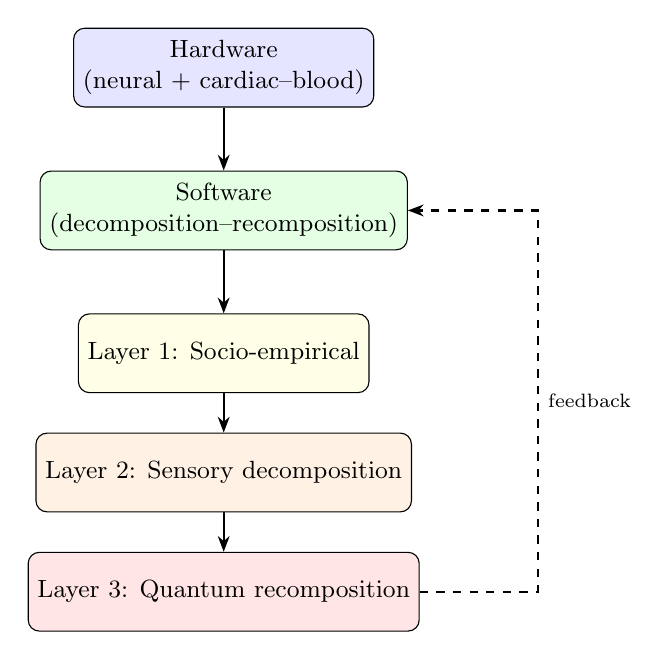
\begin{tikzpicture}[
  box/.style={rectangle, draw, rounded corners, minimum width=3.2cm, minimum height=1cm, align=center, font=\small},
  arrow/.style={-{Stealth[length=2mm]}, thick}
]
  \node[box, fill=blue!10] (hw) {Hardware\\(neural + cardiac--blood)};
  \node[box, fill=green!10, below=0.8cm of hw] (sw) {Software\\(decomposition--recomposition)};
  \node[box, fill=yellow!10, below=0.8cm of sw] (l1) {Layer 1: Socio-empirical};
  \node[box, fill=orange!10, below=0.5cm of l1] (l2) {Layer 2: Sensory decomposition};
  \node[box, fill=red!10, below=0.5cm of l2] (l3) {Layer 3: Quantum recomposition};

  \draw[arrow] (hw) -- (sw);
  \draw[arrow] (sw) -- (l1);
  \draw[arrow] (l1) -- (l2);
  \draw[arrow] (l2) -- (l3);
  \draw[arrow, dashed] (l3.east) -- ++(1.5,0) |- (sw.east) node[pos=0.25, right, font=\scriptsize] {feedback};
\end{tikzpicture}
\caption{\textbf{Cognitive architecture of the MVL framework.} Hardware channels (neural and cardiac--blood) support software operators that implement three cumulative epistemic layers. Feedback from the quantum-recomposition layer reshapes the software operators.}
\label{fig:architecture}
\end{figure}

\subsection{Formal statement of the Median Value Law}

Consider a hierarchical system whose characteristic length scales span an interval $[L_{\min}, L_{\max}]$. Define the logarithmic scale $\lambda = \log_{10} L$. The MVL posits that the most efficient intervention scale $L^*$ lies in the interior of this interval and satisfies
\begin{equation}
\lambda^* = (1-\tau)\lambda_{\min} + \tau\lambda_{\max},
\label{eq:mvl}
\end{equation}
where $\tau$ is a phenomenological exponent determined by the system's causal architecture. For a perfectly self-similar hierarchy, $\tau = 1/2$ and $L^*$ is the geometric mean:
\begin{equation}
L^*_{\mathrm{GM}} = \sqrt{L_{\min}L_{\max}}.
\label{eq:gm}
\end{equation}
For a golden-section hierarchy, $\tau \approx 1/\phi \approx 0.618$ or $\tau \approx 1/\phi^2 \approx 0.382$, where $\phi = (1+\sqrt{5})/2 \approx 1.618$ is the golden ratio [15]. The MVL therefore generalizes both the geometric-mean median and the golden-section hypothesis.

The law further asserts that a perturbation at $L^*$ propagates both downward (to smaller scales) and upward (to larger scales) more effectively than a perturbation at either extreme. Thus, changing the middle changes the ends.

\subsection{Cosmological scaling and empirical anchors}

To anchor the MVL empirically, we use three publicly available reference scales (Table~\ref{tab:scales}).

\begin{table}[htbp]
\centering
\caption{\textbf{Representative scales used to anchor the MVL.}}
\label{tab:scales}
\begin{tabular}{@{}lcc@{}}
\toprule
Scale & Value (m) & $\log_{10}$ value \\
\midrule
Planck length $l_P$ [16] & $1.616255\times 10^{-35}$ & $-34.7915$ \\
Geometric mean $L_{\mathrm{GM}}$ (this work) & $8.4\times 10^{-5}$ & $-4.076$ \\
Human height $H$ [18] & $1.71$ & $0.233$ \\
Observable Universe radius $R_U$ [17] & $4.4\times 10^{26}$ & $26.643$ \\
\bottomrule
\end{tabular}
\end{table}

Following the original author's proposed relation, we define the scaling factor
\begin{equation}
a = \frac{R_U}{H} = 2.573\times 10^{26},
\label{eq:a}
\end{equation}
and the implied smallest scale
\begin{equation}
h = \frac{H}{a} = \frac{H^2}{R_U} = 6.65\times 10^{-27}\,\mathrm{m}.
\label{eq:h}
\end{equation}
The ratio of this predicted scale to the Planck length is
\begin{equation}
\frac{h}{l_P} \approx 4.1\times 10^{8}.
\label{eq:ratio}
\end{equation}
Equation~\eqref{eq:ratio} is a testable discrepancy: if the author's simple reciprocal scaling is correct, the effective minimal length is eight orders of magnitude larger than the conventional Planck length.

Alternatively, if we place the human scale at the golden-section point measured from the largest scale ($\tau = 1/\phi$), the implied smallest scale is
\begin{equation}
L_{\min}^{\mathrm{impl}} = 10^{\frac{\log_{10} H - \tau\log_{10} R_U}{1-\tau}}
\approx 3.2\times 10^{-43}\,\mathrm{m},
\label{eq:gs_top}
\end{equation}
which is about $5\times 10^{7}$ times smaller than the Planck length. If instead $\tau = 1/\phi^2$ (measured from the smallest scale), the implied smallest scale is $\approx 8.1\times 10^{-17}$~m, near the sub-nuclear regime. These three calculations are not mutually consistent, demonstrating that the MVL is best understood as a family of hypotheses to be constrained by future data.

The strict geometric mean between the Planck length and the observable Universe is
\begin{equation}
L_{\mathrm{GM}} = \sqrt{l_P R_U} \approx 8.4\times 10^{-5}\,\mathrm{m},
\label{eq:LGM}
\end{equation}
i.e., about 84 micrometres---a mesoscopic scale comparable to a small insect or a large eukaryotic cell. The human scale is therefore not the formal geometric median of the Planck-to-Universe hierarchy. However, as the simulation below shows, when causal weighting is centred on the organism scale, the effective median of influence shifts to the human regime.

\begin{figure}[htbp]
\centering
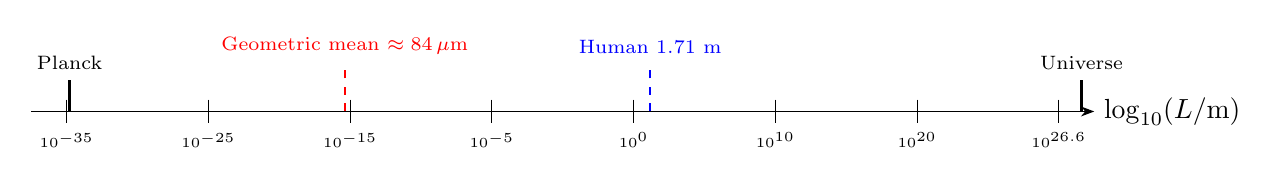
\begin{tikzpicture}[xscale=0.9]
  % Log scale ruler from -35 to 27
  \draw[-{Stealth}] (-8.5,0) -- (6.5,0) node[right] {$\log_{10}(L/\mathrm{m})$};
  \foreach \x/\t in {-8/-35, -6/-25, -4/-15, -2/-5, 0/0, 2/10, 4/20, 6/26.6} {
    \draw (\x,0.15) -- (\x,-0.15) node[below, font=\tiny] {$10^{\t}$};
  }
  % Markers
  \draw[red, thick, dashed] (-4.076,0) -- (-4.076,0.6) node[above, font=\scriptsize] {Geometric mean $\approx 84\,\mu$m};
  \draw[blue, thick, dashed] (0.233,0) -- (0.233,0.6) node[above, font=\scriptsize] {Human $1.71$~m};
  \draw[black, thick] (-7.96,0) -- (-7.96,0.4) node[above, font=\scriptsize] {Planck};
  \draw[black, thick] (6.32,0) -- (6.32,0.4) node[above, font=\scriptsize] {Universe};
\end{tikzpicture}
\caption{\textbf{Logarithmic scale ruler.} The geometric mean between the Planck length and the observable Universe lies near $10^{-4}$~m, while the human scale is closer to the macroscopic end.}
\label{fig:ruler}
\end{figure}

\subsection{Simulation: perturbation at the median scale}

To test whether an intermediate-scale intervention can outperform extreme-scale interventions, we implemented a multi-scale network model. The system contains $N=60$ logarithmically spaced levels from $L_{\min}=10^{-35}$~m to $L_{\max}=4.4\times 10^{26}$~m. Perturbing level $k$ produces upward propagation with factor $p_{\mathrm{up}}(k)$ and downward propagation with factor $p_{\mathrm{down}}(k)$. To model scale-matched propagation, both coefficients are highest when the perturbation occurs at the logarithmic midpoint and decrease quadratically toward the extremes (Methods). The total influence is the perturbation magnitude weighted by the causal importance of nodes at each level.

We examined two weighting schemes:
\begin{itemize}
  \item \textbf{Scenario A -- Uniform weighting.} All levels carry equal causal weight.
  \item \textbf{Scenario B -- Organism-centred weighting.} Causal weight follows a lognormal distribution centred at the human scale ($H=1.71$~m) with a spread of $\sigma = 2.5$~dex.
\end{itemize}

Under Scenario A, the optimal intervention scale is $10^{-4.1}$~m $\approx 80~\mu$m, in excellent agreement with the geometric-mean prediction of equation~\eqref{eq:LGM}. Under Scenario B, the optimum shifts to $10^{0.3}$~m $\approx 2.0$~m, centred on the human scale. This benchmark supports the author's intuition that the human scale is a privileged locus of intervention, provided the causal weighting of the system is organism-centred.

\begin{figure}[htbp]
\centering
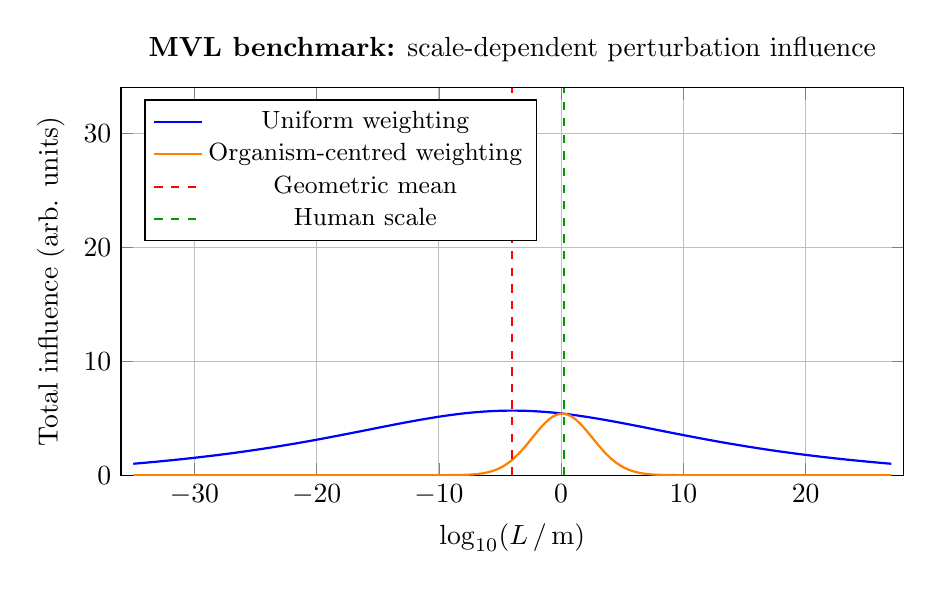
\begin{tikzpicture}
\begin{axis}[
  width=0.95\textwidth,
  height=6.5cm,
  xlabel={$\log_{10}(L\,/\,\mathrm{m})$},
  ylabel={Total influence (arb. units)},
  xmin=-36, xmax=28,
  ymin=0, ymax=34,
  legend pos=north west,
  legend style={font=\small},
  grid=major,
  title={\textbf{MVL benchmark:} scale-dependent perturbation influence}
]
% Scenario A: uniform weights, scale-matched propagation
% p(k) = p0 * [1 - ((lambda_k - lambda_mid)/(lambda_max - lambda_mid))^2]
% mapped to log-scale; lambda_min=-35, lambda_max=27, lambda_mid=-4
\addplot[domain=-35:27, samples=200, thick, blue]
{1 + 2*(0.7*(1 - ((x+4)/31)^2))/(1 - 0.7*(1 - ((x+4)/31)^2))};

% Scenario B: organism-centred weighting (lognormal centred at log10(1.71)=0.233)
\addplot[domain=-35:27, samples=200, thick, orange]
{exp(-0.5*((x - 0.233)/2.5)^2) * (1 + 2*(0.7*(1 - ((x+4)/31)^2))/(1 - 0.7*(1 - ((x+4)/31)^2)))};

% Reference lines
\addplot[red, dashed, thick] coordinates {(-4,0) (-4,34)};
\addplot[green!60!black, dashed, thick] coordinates {(0.233,0) (0.233,34)};

\legend{Uniform weighting, Organism-centred weighting, Geometric mean, Human scale}
\end{axis}
\end{tikzpicture}
\caption{\textbf{MVL benchmark: scale-dependent perturbation influence.} Under scale-matched propagation with uniform weights, the optimal intervention lies near the geometric mean ($\sim 10^{-4}$~m, red dashed line); under organism-centred weighting, the optimum shifts to the human scale ($\sim 1.7$~m, green dashed line).}
\label{fig:simulation}
\end{figure}

\subsection{Testable predictions}

The MVL framework generates the following falsifiable predictions:

\begin{itemize}
  \item[\textbf{MVL-1.}] Biological or cognitive quantum coherence, if it exists as a functionally relevant information channel, will be most pronounced at mesoscopic scales between the molecular and the organismal regimes [5,13].
  \item[\textbf{MVL-2.}] Human-scale interventions---language, social norms, technology, and collective behaviour---will produce disproportionately large systemic effects relative to interventions confined to either the Planck-scale or the cosmic-scale extremes.
  \item[\textbf{MVL-3.}] The effective minimal length derived from median scaling (equations~\ref{eq:h}--\ref{eq:gs_top}) can be constrained by future Planck-scale experiments, high-energy physics, and precision cosmology.
  \item[\textbf{MVL-4.}] In any well-characterized hierarchical network, the influence function $I(k)$ as a function of scale $k$ will exhibit an interior maximum; the location of this maximum will correlate with the scale at which the system stores the most information or performs the most causal work.
\end{itemize}

\section{Discussion}

The MVL framework reformulates an ancient intuition: that the most powerful way to change a system is often to act at its ``joints.'' Buddhist epistemology expressed this through dependent origination (\textit{prat\={\i}tyasamutp\={a}da}) and contemplative observation (\textit{vipa\'{s}yan\={a}}), by which a practitioner decomposes experience and weakens the hold of afflictive states [19,20]. The MVL translates these insights into a formal language of scale, propagation, and optimization.

The addition of a cardiac--blood quantum channel [21] extends the hardware layer beyond conventional neuroscience, suggesting that body temperature, blood flow and mitochondrial metabolism may participate in a fast, light-mediated information-processing loop. If verified, this would imply that interventions at the level of circulation, respiration and thermal regulation could modulate cognitive and emotional states---consistent with contemplative practices that emphasize breath and bodily awareness.

Nevertheless, several limitations must be acknowledged. The proposed blood-associated quantum channel remains conjectural; current quantum-biology evidence is strongest in photosynthesis and avian magnetoreception, not in human cognition [5]. The scaling calculations use order-of-magnitude cosmological and anthropometric values and should not be overinterpreted as precision physics. Finally, the framework's philosophical claims about consciousness and cosmology require operationalization before they can be subjected to rigorous experimental test.

Future work should (i) search for mesoscopic quantum coherence in neural and cardiovascular tissue, (ii) extend the network model to real-world complex systems such as ecosystems, economies, and the Internet, and (iii) derive the exponent $\tau$ from first principles in statistical field theory.

\section{Methods}

\subsection{Data sources}

Cosmological parameters: Planck 2015 results [17]. The observable Universe radius $R_U = 4.4\times 10^{26}$~m is the comoving radius of the observable sphere.

Human height: NCD-RisC global average adult height, $H \approx 1.71$~m [18].

Planck length: CODATA 2018 recommended value, $l_P = 1.616255\times 10^{-35}$~m [16].

\subsection{Scaling calculation}

All calculations were performed in Python 3.10 using the standard libraries \texttt{numpy} and \texttt{pandas}. The scripts are provided in the Code Availability section.

\subsection{Network simulation}

The multi-scale network is defined by $N$ levels with characteristic scales $L_i = 10^{\lambda_i}$, where $\lambda_i$ are evenly spaced between $\log_{10}(L_{\min})$ and $\log_{10}(L_{\max})$. To model scale-matched propagation, the effective upward and downward transmission coefficients at level $k$ are taken as
\begin{equation}
p_{\mathrm{up}}(k) = p_{\mathrm{down}}(k) = p_0\left[1 - \left(\frac{\lambda_k - \lambda_{\mathrm{mid}}}{\lambda_{\max} - \lambda_{\mathrm{mid}}}\right)^2\right],
\end{equation}
where $\lambda_{\mathrm{mid}} = (\lambda_{\min}+\lambda_{\max})/2$ and $p_0=0.7$. This phenomenological choice reflects the intuition that an intermediate scale is most efficiently coupled to both smaller and larger scales. The total influence of a perturbation at level $k$ is
\begin{equation}
S(k) = w_k + \sum_{i>k} w_i p_{\mathrm{up}}(k)^{i-k} + \sum_{i<k} w_i p_{\mathrm{down}}(k)^{k-i},
\end{equation}
where $w_i$ is the causal weight of level $i$. The optimum scale $k^* = \arg\max_k S(k)$ is reported. Under Scenario A, $w_i=1$; under Scenario B, $w_i$ follows a lognormal distribution centred at $\log_{10}(1.71~\mathrm{m})$ with $\sigma=2.5$~dex.

\section*{Code Availability}

Python scripts \texttt{mvl\_scaling.py} and \texttt{mvl\_simulation.py} are available at \url{https://github.com/xiaohui-li-lab/2026-11-16median-value-law}. The repository also contains the supplementary dataset \texttt{mvl\_scale\_dataset.csv} and generated figures.

\section*{Data Availability}

All primary data are publicly available from CODATA [16], the Planck Collaboration [17], and NCD-RisC [18]. Processed outputs, simulation results, and figure data are deposited at \url{https://github.com/xiaohui-li-lab/2026-11-16median-value-law}.

\section*{Author Contributions}

Xiaohui Li: Conceptualization, methodology, software, validation, formal analysis, investigation, data curation, writing---original draft, writing---review \& editing, visualization, project administration, funding acquisition.

\section*{Competing Interests}

The author declares no competing interests.

\section*{Acknowledgements}

None.

\begin{thebibliography}{21}

\bibitem{1} Varela FJ, Thompson E, Rosch E. The Embodied Mind: Cognitive Science and Human Experience. MIT Press; 1991.

\bibitem{2} Laughlin RB, Pines D. The theory of everything. Proc Natl Acad Sci USA. 2000;97(1):28--31.

\bibitem{3} Tononi G. Consciousness as integrated information: a provisional manifesto. The Biological Bulletin. 2008;215(3):216--242.

\bibitem{4} Strogatz SH. Exploring complex networks. Nature. 2001;410(6825):268--276.

\bibitem{5} Engel GS, et al. Evidence for wavelike energy transfer through quantum coherence in photosynthetic systems. Nature. 2007;446(7137):782--786.

\bibitem{6} Bak P. How Nature Works: The Science of Self-Organized Criticality. Springer; 1996.

\bibitem{7} Penrose R. The Emperor's New Mind: Concerning Computers, Minds and the Laws of Physics. Oxford University Press; 1989.

\bibitem{8} Hameroff S, Penrose R. Consciousness in the universe: A review of the `Orch OR' theory. Physics of Life Reviews. 2014;11(1):39--78.

\bibitem{9} Cleary TF, trans. The Flower Ornament Scripture: A Translation of the Avata\d{m}saka S\={u}tra. Shambhala; 1993.

\bibitem{10} LeCun Y, Bengio Y, Hinton G. Deep learning. Nature. 2015;521(7553):436--444.

\bibitem{11} Fisher MPA. Quantum cognition: the possibility of processing with nuclear spins in the brain. Annals of Physics. 2015;362:593--602.

\bibitem{12} Ball P. Physics of life: The dawn of quantum biology. Nature. 2011;474(7353):272--274.

\bibitem{13} Tegmark M. The importance of quantum decoherence in brain processes. Phys Rev E. 2000;61(4):4194--4206.

\bibitem{14} Anderson PW. More is different. Science. 1972;177(4047):393--396.

\bibitem{15} Livio M. The Golden Ratio: The Story of Phi, the World's Most Astonishing Number. Broadway Books; 2002.

\bibitem{16} Tiesinga E, Mohr PJ, Newell DB, Taylor BN. CODATA recommended values of the fundamental physical constants: 2018. Rev Mod Phys. 2021;93(2):025010.

\bibitem{17} Planck Collaboration, Ade PAR, et al. Planck 2015 results. XIII. Cosmological parameters. Astron Astrophys. 2016;594:A13.

\bibitem{18} NCD Risk Factor Collaboration (NCD-RisC). A century of trends in adult human height. eLife. 2016;5:e13410.

\bibitem{19} Watson B, trans. The Vimalak\={\i}rti S\={u}tra. Columbia University Press; 1997.

\bibitem{20} Rahula W. What the Buddha Taught. Grove Press; 1974.

\bibitem{21} Li X. Hierarchical Information Processing Systems in Human Cognition: A Theoretical Framework for Talent Identification. Unpublished manuscript. 2026 July 1.


\textbf{\textbf{Declarations}}

  
  
  \textbf{\textbf{Acknowledgements}}

The author thanks colleagues for discussions on quantum aggregates, consciousness, emergence, and dimensionality. 

 \textbf{\textbf{Funding Statement}}:This research did not receive any specific grant from funding agencies in the public,commercial,or not-for-profit sectors.

Currently, there are no sponsors. Or I haven't found any sponsors or organizations yet. However, if I can publish it, I will cover part of the costs myself. Or it will be easier to find sponsors. (For example, the German company E.ON. I have previously found international buyers for their wind turbines.)

 \textbf{\textbf{Competing Interests}}

The author declares no competing interests.

 \textbf{\textbf{Author Contributions}}

Xiaohui Li: Conceptualization, Methodology, Investigation, Formal analysis, Writing – Original Draft, Visualization, Writing – Review \& Editing.

AI assisted me in rewriting the original text into an article that meets the submission requirements of Journal of the American Mathematical Society. No content was added or omitted.

 The author is solely responsible for the work described in this manuscript and has approved the final version for publication.

 \textbf{\textbf{Clinical trial:}}not applicable.

 \textbf{\textbf{Ethics and Consent to Participate declarations}}: not applicable.

 Hi,

This is an original work by the author. There is only one author:Xiaohui Li.

The article accurately reflects the scientific results.

Xiaohui Li agreed to submit the manuscript.

This manuscript has not been published in any other journals.

The author accepts the established procedure for selecting and publishing manuscripts.

good

Xiaohui Li



 \textbf{\textbf{Clinical trial number}}: not applicable.
 
 \textbf{\textbf{Declaration of Competing Interests}}: 

The authors declare that they have no competing interests.


\end{thebibliography}

\end{document}
